%%********************Chapter 4**********
\chapter{\uppercase{Objectives and Proposed System}}

\section{Objectives}
The main objectives of the proposed project are:
\begin{enumerate}
	\item To design a mobile application that allows users to define financial goals with a target amount and time horizon such as retirement, education, or vehicle purchase.
	\item To develop a risk-profiling module that assesses both risk tolerance and risk capacity based on the user's goal horizon and financial situation.
	\item To build a recommendation engine inspired by the base paper's regret-optimized and future-looking reward formulation that dynamically adjusts asset allocation across mutual funds, equity, and debt instruments as the goal's deadline approaches.
	\item To provide an intuitive mobile dashboard for tracking goal progress, required SIP contributions, and recommended portfolio adjustments over time.
\end{enumerate}

\section{System Requirements}

\begin{table}[h!]
	\centering
	\caption{Functional Requirements of the Proposed System}
	\label{tab:funcreq}
	\vspace*{5pt}
	{\singlespacing\small
	\begin{tabular}{|c|p{4cm}|p{6.5cm}|}
		\hline
		\textbf{No.} & \textbf{Requirement} & \textbf{Description} \\ \hline
		1 & Goal Creation & User can create a financial goal with target amount and time horizon. \\ \hline
		2 & Financial Calculation & System calculates required savings and periodic investment. \\ \hline
		3 & Risk Profiling & System evaluates user risk tolerance and risk capacity. \\ \hline
		4 & Feasibility Assessment & System checks whether the selected goal is financially achievable. \\ \hline
		5 & Investment Recommendation & System provides personalized investment allocation recommendations. \\ \hline
		6 & Dynamic Allocation & System adjusts allocation based on remaining goal horizon. \\ \hline
		7 & Progress Tracking & User can monitor goal progress through the mobile dashboard. \\ \hline
	\end{tabular}}
\end{table}

\subsection{Functional Requirements}
The proposed system shall provide the following functional capabilities:
\begin{itemize}
	\item User profile management.
	\item Financial goal creation and management.
	\item Goal amount and deadline input.
	\item Inflation-adjusted goal calculation.
	\item SIP calculation.
	\item Safety and feasibility assessment.
	\item Risk profiling.
	\item Personalized investment recommendation.
	\item Dynamic asset allocation.
	\item Goal progress tracking.
	\item Mobile dashboard.
\end{itemize}

\subsection{Non-Functional Requirements}
The system should satisfy the following non-functional requirements:
\begin{itemize}
	\item Usability.
	\item Reliability.
	\item Security.
	\item Maintainability.
	\item Scalability.
	\item Performance.
	\item Responsiveness.
\end{itemize}

\subsection{Software Requirements}
The planned software environment includes:
\begin{itemize}
	\item Mobile application development framework.
	\item Backend and API services.
	\item Database system.
	\item Python-based machine-learning environment.
	\item Reinforcement Learning libraries.
	\item Development and testing tools.
\end{itemize}

\section{Proposed System Architecture}
The proposed system architecture illustrates the overall workflow of the Financial Goal Planner and the interaction between its major modules. The system collects the user's financial goal, target amount, investment horizon, savings capacity, and risk-related information through the mobile application.

The collected information is processed through the Goal Management, Financial Calculation, Safety and Feasibility, and Risk Profiling modules. These outputs are provided to the Recommendation Engine, which generates a personalized investment recommendation based on the user's goal, financial condition, risk profile, and investment horizon.

The Dynamic Allocation Module adjusts the recommended allocation according to the remaining goal horizon. Finally, the Dashboard presents the goal progress, financial requirements, feasibility status, risk profile, and recommended allocation to the user.

\begin{figure}[h!]
	\centering
	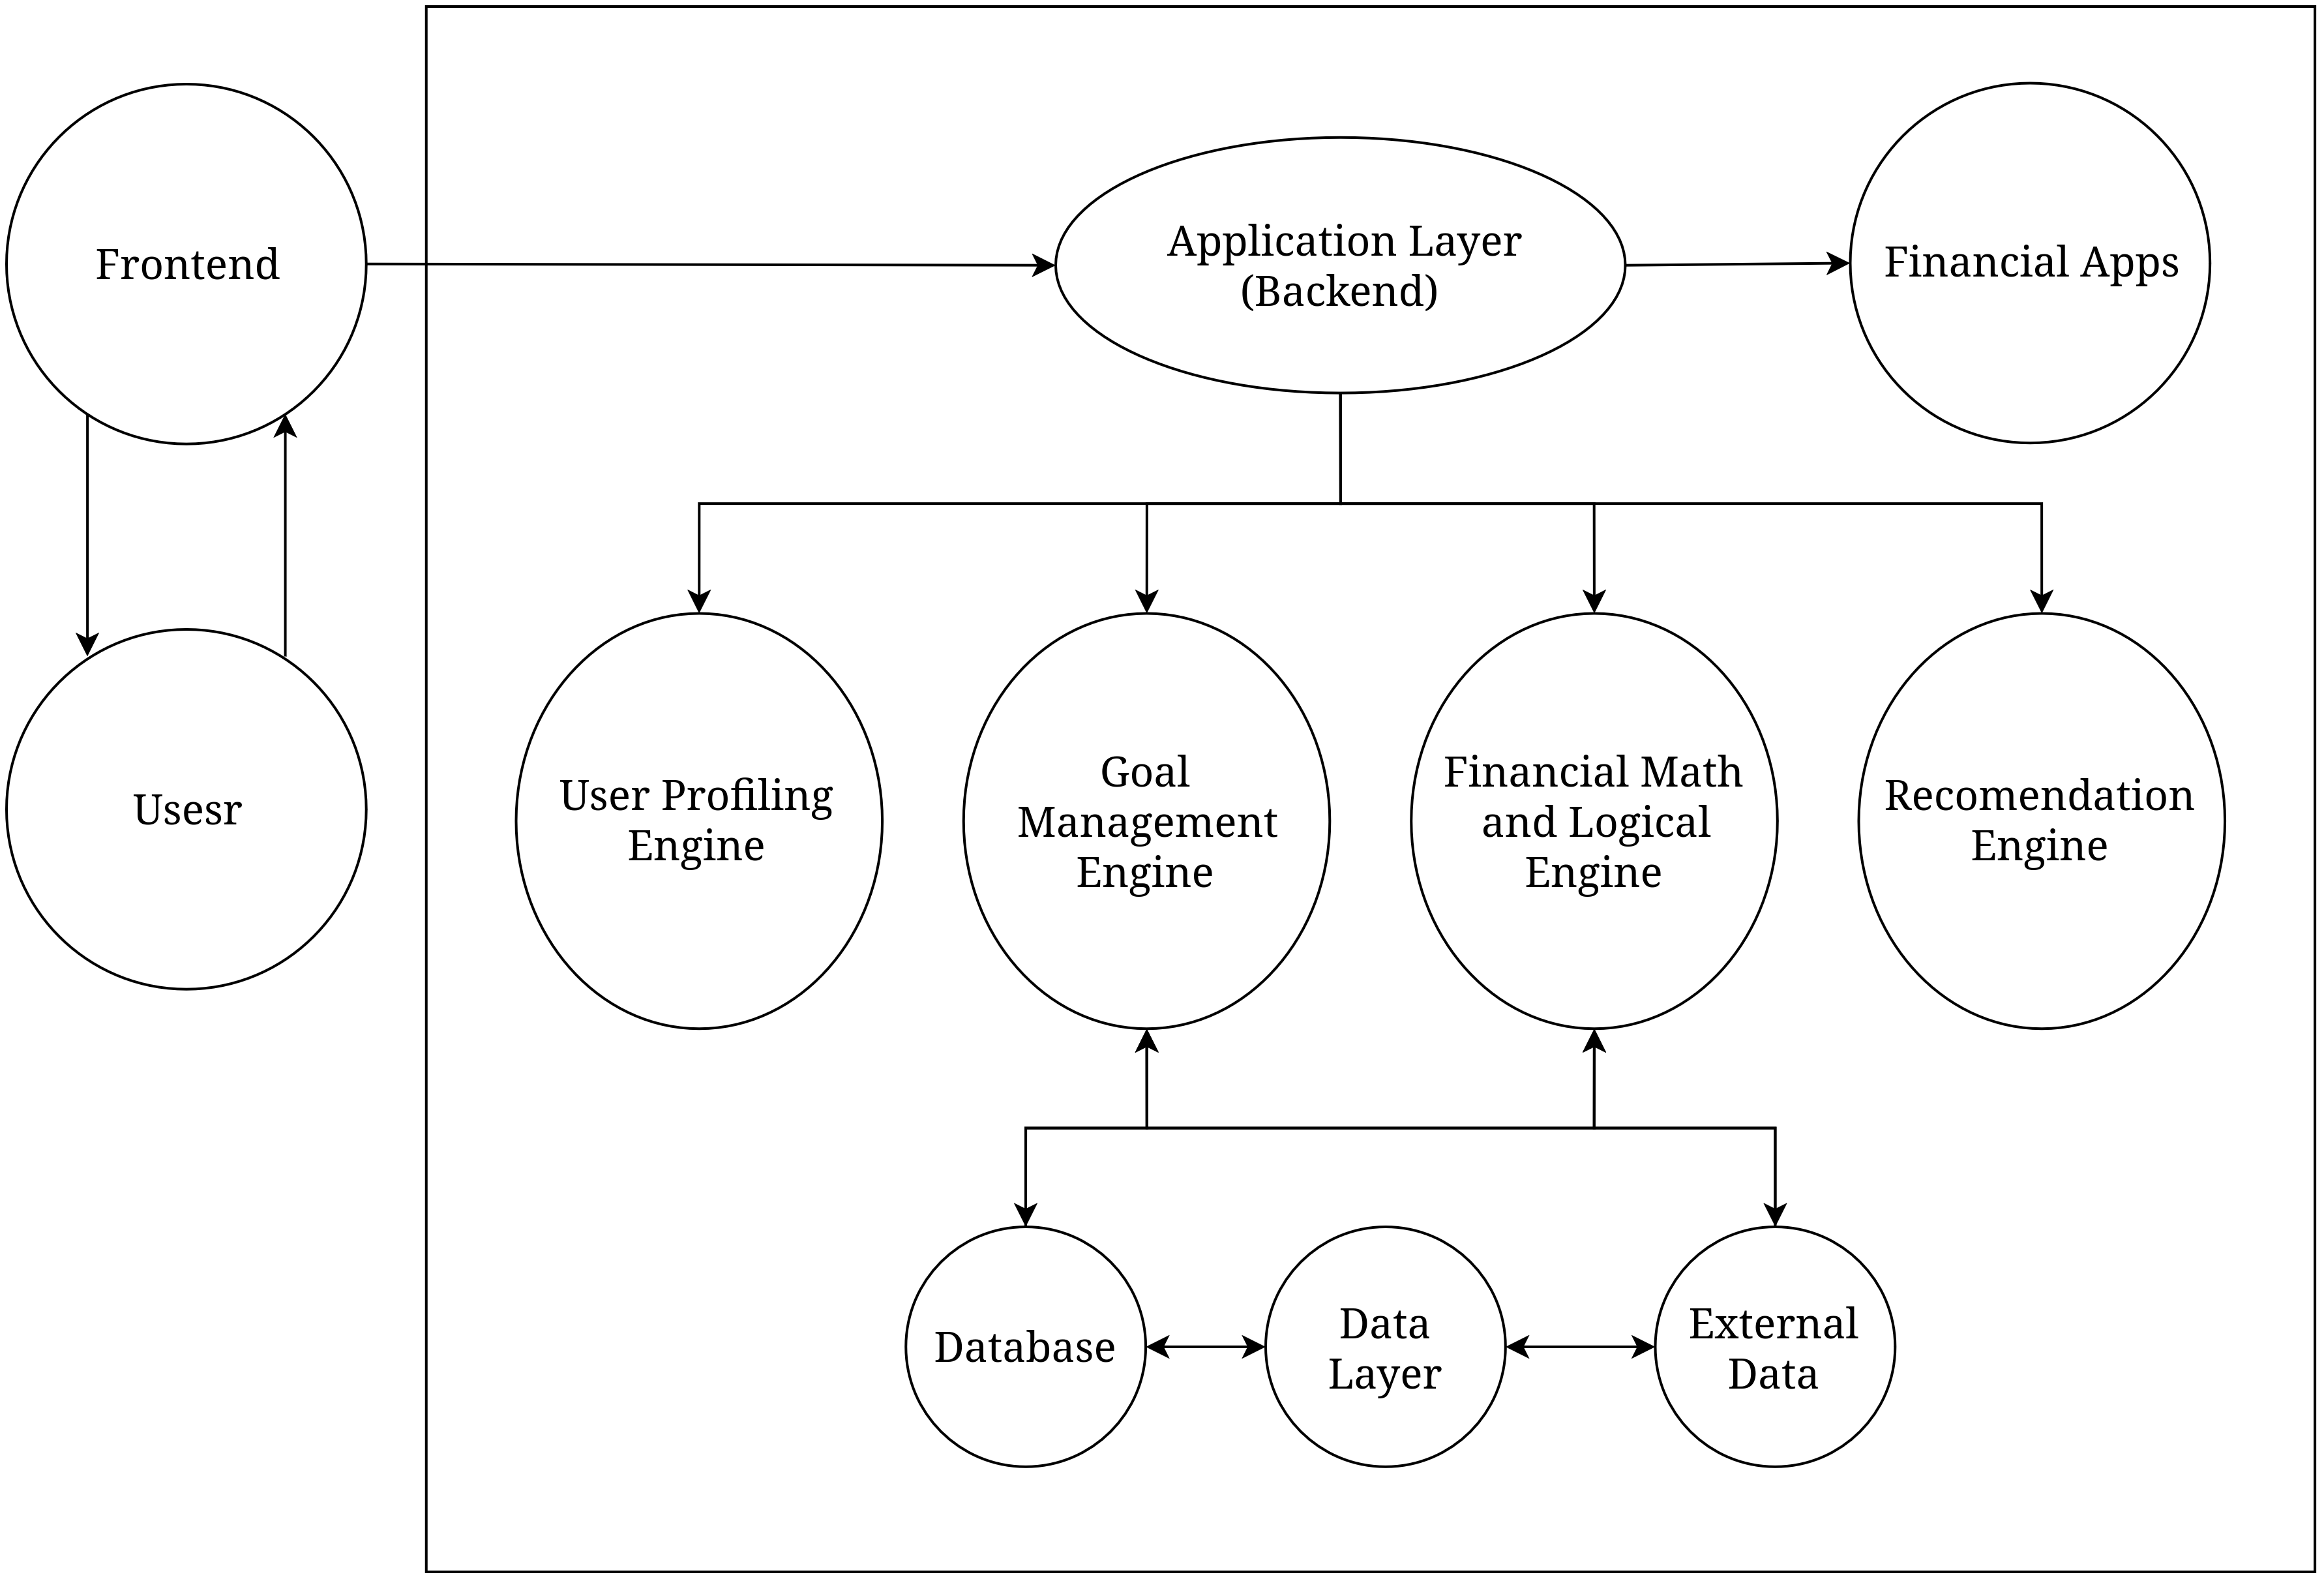
\includegraphics[width=0.95\linewidth]{figures/architecture.png}
	\caption{Proposed System Architecture}
	\label{fig:architecture}
\end{figure}

The proposed architecture is inspired by the base paper, ``Regret-Optimized Portfolio Enhancement through Deep Reinforcement Learning and Future Looking Rewards''. The proposed system adapts the regret-aware and future-looking portfolio concepts to a goal-based financial planning environment by considering the financial goal, feasibility, risk profile, and remaining investment horizon.
\subsection{Process Diagram}

The process diagram illustrates the overall sequence of operations
performed by the proposed Financial Goal Planner. It represents how
the user's goal, financial information, and risk-related information
are processed through the different modules to generate a
personalized investment recommendation.

The process begins when the user provides the required goal,
financial, and risk-related information through the mobile
application. The Goal Management module processes the goal-related
information such as the target amount and investment horizon.

After goal information is processed, the system performs two major
activities. The Financial Calculation module calculates the
financial requirements of the selected goal, including inflation
adjustment, required savings, and SIP contribution. At the same time,
the Risk Profiling module analyses the user's risk-related
information to determine risk tolerance and risk capacity.

The output of the Financial Calculation module is provided to the
Safety and Feasibility Calculator, which evaluates whether the
selected financial goal is practically achievable based on the
user's financial capacity. The outputs from the feasibility
assessment and Risk Profiling module are then combined with the
financial and goal-related information.

These inputs are provided to the Recommendation Engine, which
generates a personalized investment recommendation based on the
user's financial goal, financial condition, risk profile, and
investment horizon. The Dynamic Allocation module subsequently
adjusts the recommended asset allocation according to the remaining
goal horizon and the user's risk characteristics.

Finally, the Dashboard presents the processed information to the
user, including the goal progress, required investment, feasibility
status, risk profile, and recommended asset allocation.

Thus, the process diagram provides a clear representation of the
overall workflow of the proposed Financial Goal Planner, from user
input to financial analysis, risk assessment, recommendation, and
final presentation.

\begin{figure}[H]
    \centering

    \begin{tikzpicture}[
        box/.style={
            rectangle,
            rounded corners,
            draw,
            thick,
            align=center,
            minimum width=3.8cm,
            minimum height=0.75cm,
            font=\scriptsize
        },
        arrow/.style={
            -{Latex[length=2mm]},
            thick
        }
    ]

    % Main flow
    \node[box] (user) at (0,0)
        {USER INPUT\\
        Goal + Financial + Risk Information};

    \node[box] (goal) at (0,-1.35)
        {GOAL MANAGEMENT\\
        Goal Amount + Investment Horizon};

    % Parallel modules
    \node[box] (financial) at (-2.4,-2.8)
        {FINANCIAL CALCULATION\\
        Inflation + SIP + Required Investment};

    \node[box] (risk) at (2.4,-2.8)
        {RISK PROFILING\\
        Risk Tolerance + Risk Capacity};

    % Safety
    \node[box] (safety) at (-2.4,-4.25)
        {SAFETY \& FEASIBILITY\\
        Goal Achievability};

    % Recommendation
    \node[box] (recommend) at (0,-5.7)
        {RECOMMENDATION ENGINE\\
        Personalized Investment Recommendation};

    % Dynamic allocation
    \node[box] (dynamic) at (0,-7.15)
        {DYNAMIC ALLOCATION\\
        Horizon-based Allocation Adjustment};

    % Dashboard
    \node[box] (dashboard) at (0,-8.6)
        {DASHBOARD\\
        Goal Progress + Feasibility + Risk + Recommendation};

    % Arrows
    \draw[arrow] (user) -- (goal);

    \draw[arrow] (goal.south) -- (financial.north);
    \draw[arrow] (goal.south) -- (risk.north);

    \draw[arrow] (financial.south) -- (safety.north);

    \draw[arrow] (safety.south east) -- (recommend.north west);
    \draw[arrow] (risk.south west) -- (recommend.north east);

    \draw[arrow] (recommend) -- (dynamic);
    \draw[arrow] (dynamic) -- (dashboard);

    \end{tikzpicture}

    \caption{Overall Process Flow of the Proposed Financial Goal Planner}
    \label{fig:process_diagram}

\end{figure}
\subsection{Use Case Diagram}

The Use Case Diagram represents the interaction between the user and
the major functions of the proposed Financial Goal Planner. It
identifies the main activities that can be performed by the user
through the system.

The user provides the required financial and risk-related information
through the system. The Risk Profiling and User Modelling component
collects the user's responses through a risk questionnaire and
evaluates the user's risk tolerance and risk capacity. Based on these
factors, the system classifies the user's risk profile.

The user can view the resulting risk profile and can update the
financial profile whenever the relevant financial information changes.
The resulting risk profile is later used by the Recommendation Engine
to generate a personalized investment recommendation.

\begin{figure}[H]
    \centering
	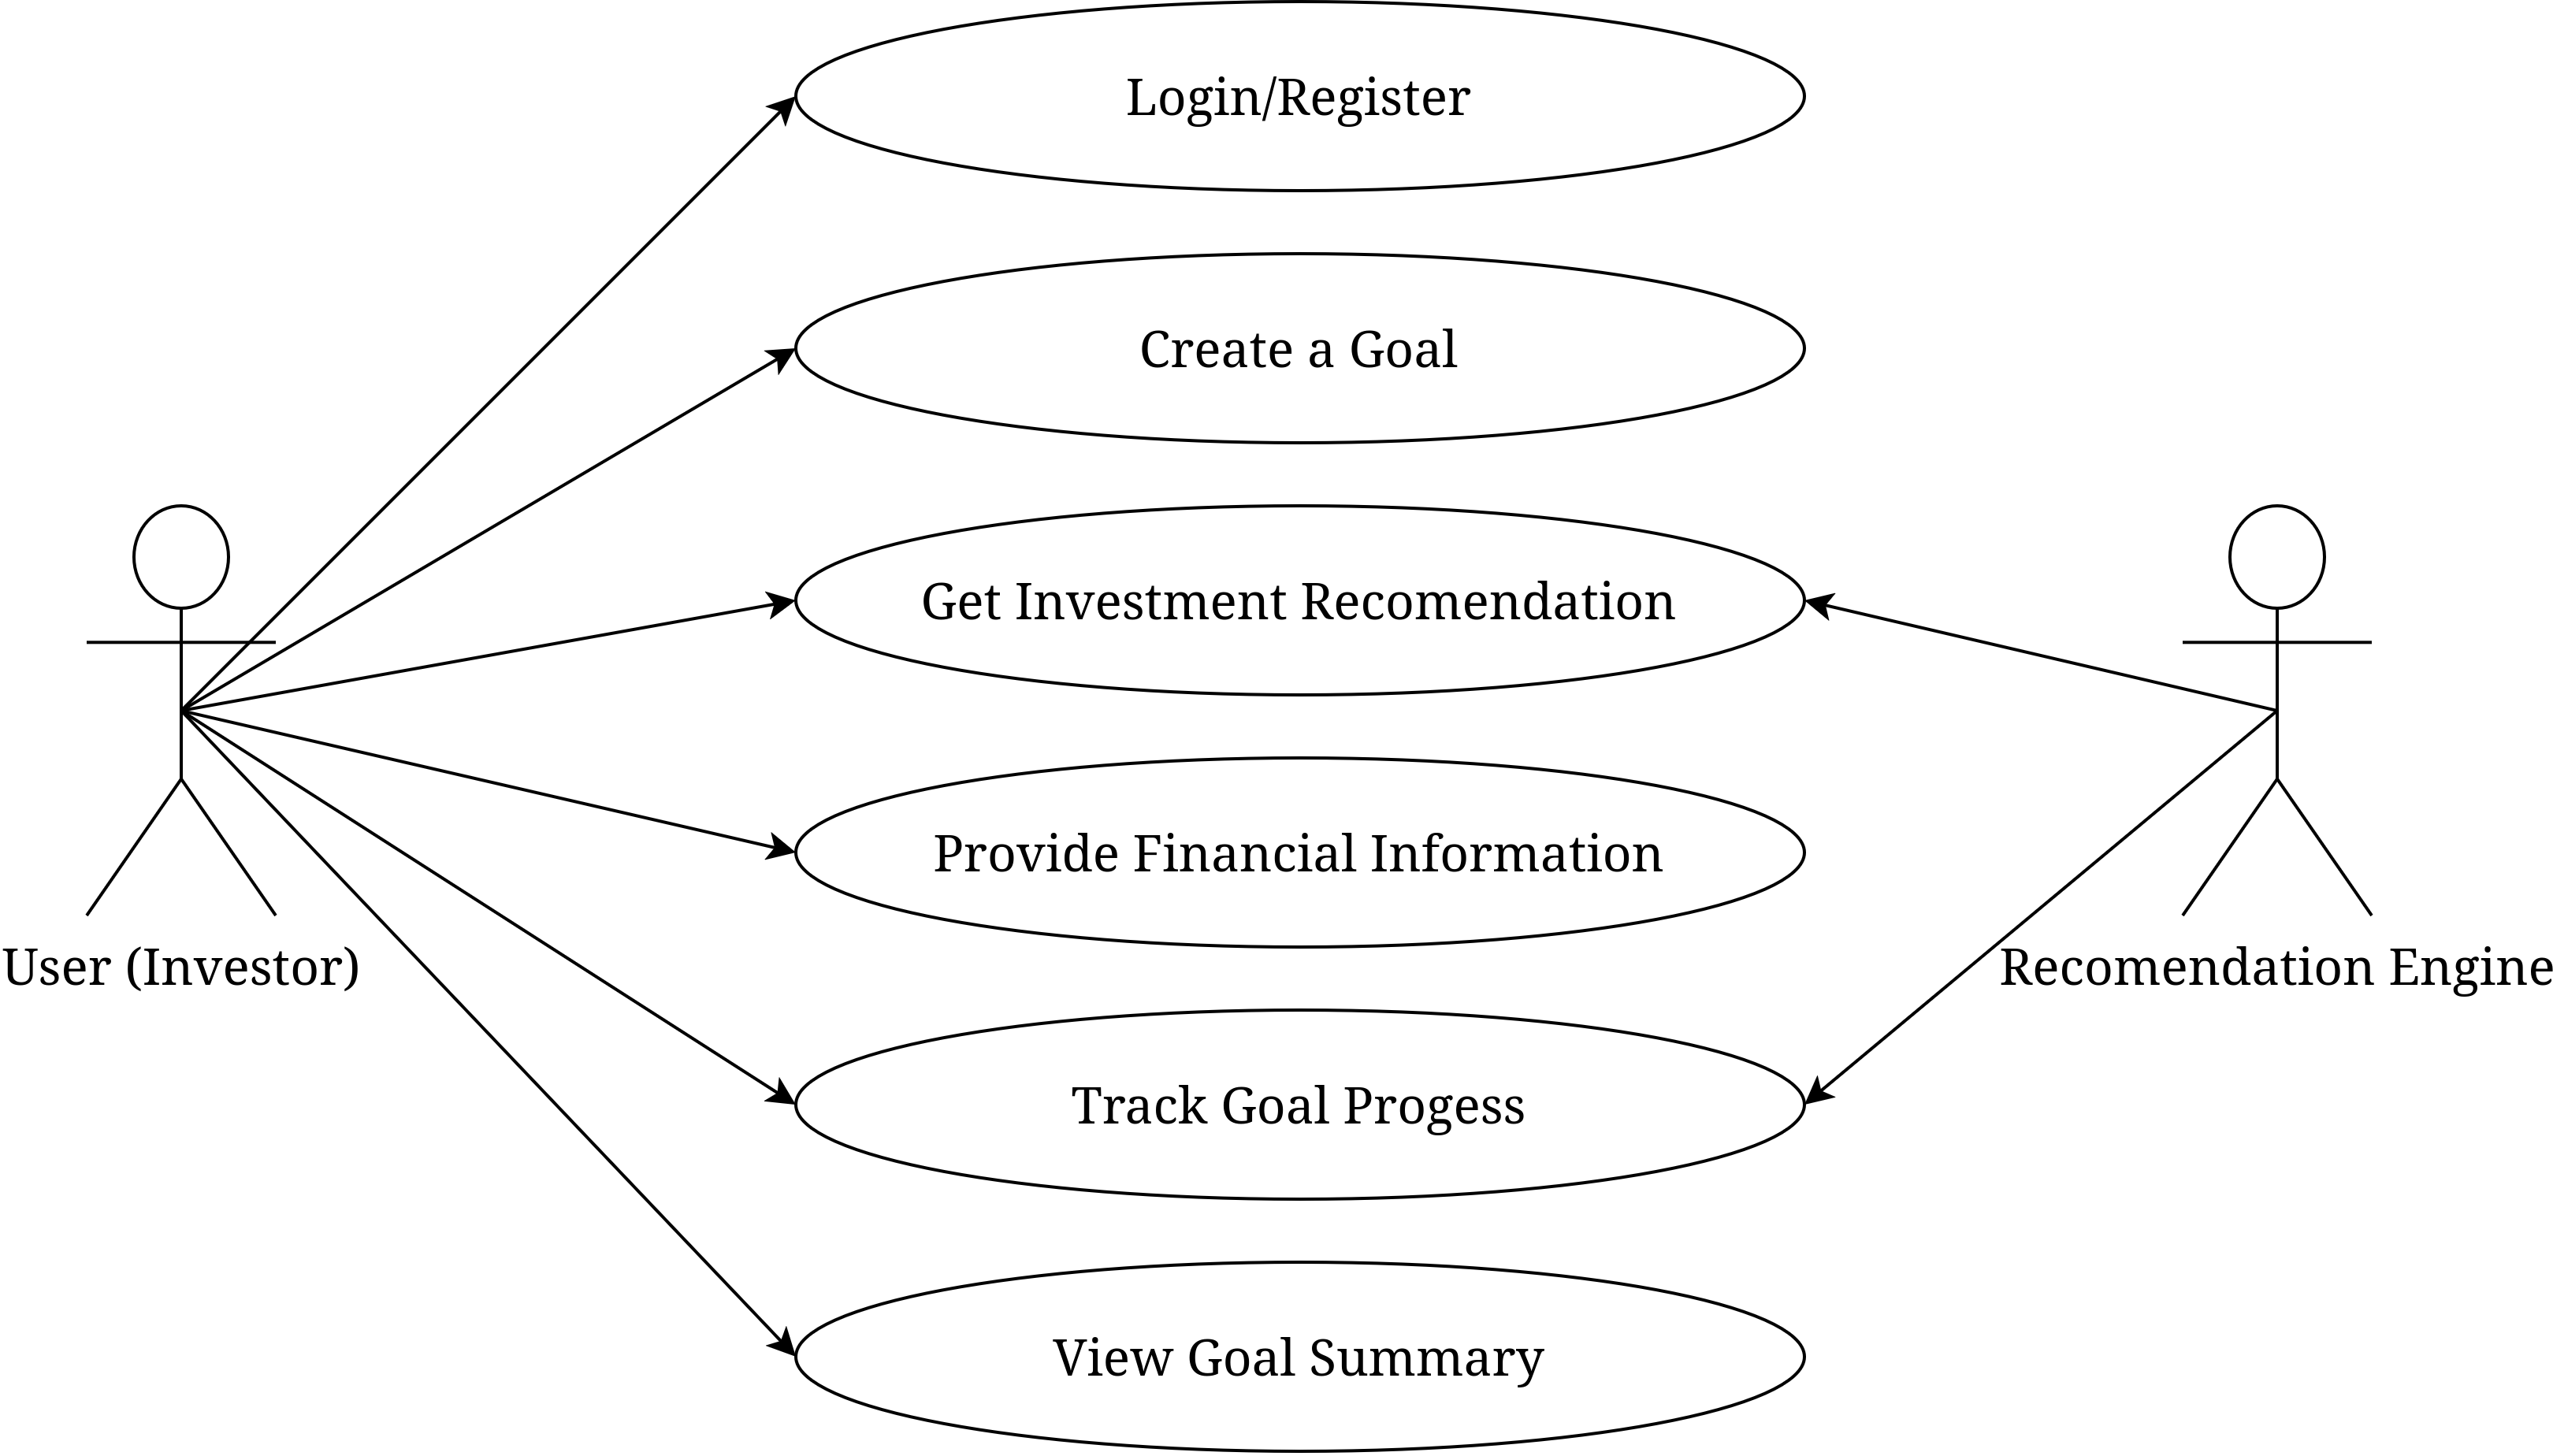
\includegraphics[width=0.95\linewidth]{figures/usecase_diagram.png}
    \caption{Use Case Diagram of the Risk Profiling and User Modelling Module}
    \label{fig:usecase_diagram}
\end{figure}

\section{Major Modules}
The proposed system consists of the following major modules, which work together to provide goal-based and risk-aware investment planning.

\subsection{Goal Management}
The Goal Management module allows users to create and manage financial goals by specifying the goal type, target amount, and investment horizon. These details are used by the subsequent financial calculation and recommendation modules.

\subsection{Financial Calculation Module}
The Financial Calculation Module determines the financial requirements associated with the selected goal. It considers factors such as target amount, investment period, inflation, expected return, and required periodic contribution such as SIP.

\subsection{Safety and Feasibility Calculator}
The Safety and Feasibility Calculator evaluates whether the selected financial goal is practically achievable. It compares the required investment with the user's available savings or periodic contribution capacity.

\subsection{Risk Profiling}
The Risk Profiling module evaluates the user's risk characteristics using relevant financial and goal-related information. The resulting risk profile is used by the Recommendation Engine while generating the investment recommendation.

\subsection{Recommendation Engine}
The Recommendation Engine combines the goal details, financial calculations, feasibility result, risk profile, and investment horizon to generate a personalized investment recommendation. Its design is inspired by the regret-based and future-looking reward concepts of the base paper.

\subsection{Dynamic Allocation and Dashboard}
The Dynamic Allocation module adjusts the recommended asset allocation according to the remaining goal horizon and the user's risk profile. The Dashboard presents the goal progress, financial requirements, feasibility status, risk profile, and recommended allocation to the user.

\begin{table}[h!]
	\centering
	\caption{Major Modules of the Proposed System}
	\label{tab:modules}
	\vspace*{5pt}
	{\singlespacing\small
	\begin{tabular}{|c|p{4cm}|p{6.5cm}|}
		\hline
		\textbf{No.} & \textbf{Module} & \textbf{Description} \\ \hline
		1 & Goal Management & Defines the financial goal, target amount, and time horizon. \\ \hline
		2 & Financial Calculation & Calculates future goal amount, required savings, and SIP contribution. \\ \hline
		3 & Safety and Feasibility & Evaluates whether the selected financial goal is practically achievable. \\ \hline
		4 & Risk Profiling & Assesses the user's risk tolerance and risk capacity. \\ \hline
		5 & Recommendation Engine & Generates personalized investment recommendations based on goal, horizon, and risk profile. \\ \hline
		6 & Dynamic Allocation and Dashboard & Adjusts asset allocation and displays goal progress and recommendations. \\ \hline
	\end{tabular}}
\end{table}

\subsection{Data Flow Diagram}
The Data Flow Diagram (DFD) represents the flow of information between the user, the external data sources and the major modules of the proposed system. It shows how the user's financial and goal-related information is processed to generate the final investment recommendation. The system is presented at two levels: Level 0 (context diagram) and Level 1 (module-level decomposition).

\subsubsection{Level 0 DFD (Context Diagram)}
The Level 0 DFD shows the Financial Goal Planner as a single process and describes its interaction with external entities. The \textbf{User} provides goal details (target amount, time horizon) and risk-profile responses, and receives the inflation-adjusted goal amount, required SIP contribution, recommended asset allocation and portfolio adjustment alerts. The \textbf{Market Data Source} (mutual fund NAV data) supplies the historical and latest market data used for growth estimation and allocation.

% Place the Level 0 DFD image at figures/level_0.png. If the file is missing,
% a placeholder box is printed instead so the document still compiles.
\begin{figure}[h!]
\centering
\IfFileExists{figures/level_0.png}{%
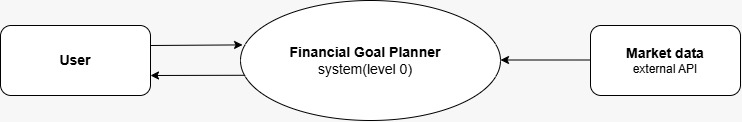
\includegraphics[width=0.95\linewidth]{figures/level_0.png}%
    }{%
\fbox{\parbox[c][7cm][c]{0.9\linewidth}{\centering DFD Level 0 --- add \texttt{figures/level\_0.png}}}%
    }
\caption{Data Flow Diagram Level 0 (Context Diagram)}
\label{fig:dfd0}
\end{figure}

\subsubsection{Level 1 DFD}
The Level 1 DFD decomposes the system into its four major modules and shows the data exchanged between them and the central database:
\begin{itemize}
    \item \textbf{Mobile Application \& UI/UX:} Accepts goal details from the user, displays the dashboard and presents recommendations.
    \item \textbf{Risk Profiling \& User Modelling:} Processes the questionnaire responses to assess risk tolerance and risk capacity, and outputs the user's risk class and financial profile.
    \item \textbf{Financial Forecasting \& Computation:} Computes the inflation-adjusted goal amount, required SIP contribution, expected investment growth and goal feasibility using processed market data.
    \item \textbf{AI Recommendation \& Portfolio Allocation:} Takes the risk profile, goal parameters and forecast results to generate the asset allocation across mutual funds, equity and debt instruments, and to adjust it as the remaining horizon shrinks.
\end{itemize}
User and goal data and generated recommendations are stored in and retrieved from the database, so that the dashboard can track goal progress over time.

% Place the Level 1 DFD image at figures/level_1.png. If the file is missing,
% a placeholder box is printed instead so the document still compiles.
\begin{figure}[h!]
\centering
\IfFileExists{figures/level_1.png}{%
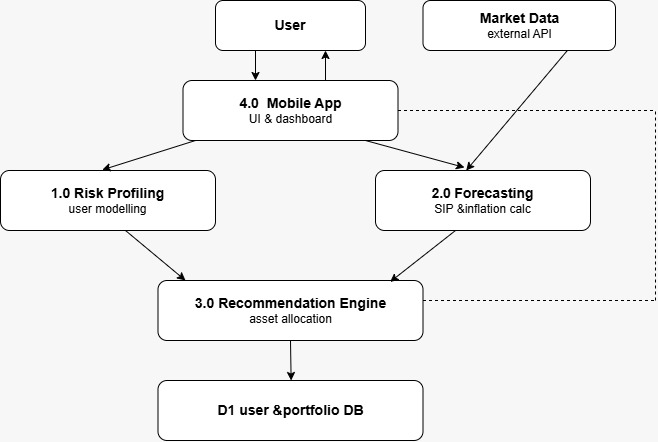
\includegraphics[width=0.95\linewidth]{figures/level_1.png}%
    }{%
\fbox{\parbox[c][7cm][c]{0.9\linewidth}{\centering DFD Level 1 --- add \texttt{figures/level\_1.png}}}%
    }
\caption{Data Flow Diagram Level 1}
\label{fig:dfd1}
\end{figure}
